\documentclass{article}

% Packages from Nicholas
\usepackage[english]{babel}
\usepackage[utf8]{inputenc}
\usepackage{fancyhdr}
\usepackage{amsmath}
\usepackage{amssymb}
\usepackage{bm}
\usepackage{geometry}
% \geometry{letterpaper}
\usepackage{amsfonts}
\usepackage{mathtools}
\usepackage{setspace}
\usepackage{makecell}
\usepackage{eurosym}
\usepackage{amstext}
\usepackage{framed}

% Inline Graphics
\usepackage{graphicx,float,subfig, grffile}
\graphicspath{{./}{figs/}}

% Captions
\usepackage[font=Large]{caption}

% Hypertext References
\usepackage{hyperref,color,textcomp}
\definecolor{webgreen}{rgb}{0,.35,0}
\definecolor{webbrown}{rgb}{.6,0,0}
\definecolor{RoyalBlue}{rgb}{0,0,0.9}
\definecolor{purp}{rgb}{0.6,0.3,0.9}
\hypersetup{
   colorlinks=true, linktocpage=true, pdfstartpage=3, pdfstartview=FitV,
   breaklinks=true, pdfpagemode=UseNone, pageanchor=true, pdfpagemode=UseOutlines,
   plainpages=false, bookmarksnumbered, bookmarksopen=true, bookmarksopenlevel=1,
   hypertexnames=true, pdfhighlight=/O,
   urlcolor=webbrown, linkcolor=RoyalBlue, citecolor=webgreen,
   pdfauthor={Nicholas Beasley, William Burke & Michael S. Emanuel},
   pdfsubject={Harvard AM205 (Fall 2018)},
   pdfkeywords={},
   pdfcreator={pdfLaTeX},
   pdfproducer={LaTeX with hyperref}
}
\hypersetup{pdftitle={AM205: Final Project}}

% Macro definitions
\newcommand{\N}{\mathbb{N}}
\newcommand{\Z}{\mathbb{Z}}
\newcommand{\Q}{\mathbb{Q}}
\newcommand{\R}{\mathbb{R}}
\newcommand{\B}{\mathbb{B}}
\newcommand{\mcL}{\mathcal{L}}
\newcommand{\p}{\partial}
\newcommand{\Trans}{\mathsf{T}}
\renewcommand{\vec}[1]{\mathbf{#1}}
\newcommand{\vx}{\vec{x}}
\newcommand{\vb}{\vec{b}}

\pagestyle{fancy}
\fancyhf{}
\chead{Basketball Motion Capture}
% \rhead{}
\rfoot{Page \thepage}
\lfoot{December 20, 2018}
\cfoot{}
\renewcommand{\headrulewidth}{0.5pt}
\renewcommand{\footrulewidth}{0.5pt}

\onehalfspacing
\begin{document}

\section*{AM 205 Final Project: Basketball Motion Capture}
\subsubsection*{
Nicholas Beasley\\
William C. Burke\\
Michael S. Emanuel}

\section{Abstract}
The goal of this project was to infer the position of a basketball in three dimensional space during a live game by obtaining multiple video recordings.
In particular, the intuition was that with enough cameras, it should be possible to construct an over-determined system and perform 
a least squares or similar style estimation of the position of the ball that is in best agreement with the video frames.
Steps we hoped to achieve in this project included 
\begin{itemize}
\item obtaining video in an experiment at the MAC; processing the video; 
\item synchronizing the video based on the audio from each clip; 
\item mapping from 3D world coordinates to 2D pixel locations on each camera;
\item tracking the ball in 2D space on each camera; 
\item inferring the position of the ball in 3D space based on its pixel location on each camera.
\item simulating the path of the ball while in flight using an extended Kalman filter and the equations of motion
\item predicting whether a shot would go in the basket at the moment it was released
\end{itemize}

When we articulated this project, we recognized that it was ambitious and that it might not be possible to do everything we wanted to
in the time available.  It has turned out that a number of the steps, while conceptually straightforward, have proven to be quite
challenging and consumed far more time than we had budgeted.  We are going to present below everything that we were able
to accomplish and hope for the forbearance of readers who are familiar with the slings and arrows of working on demanding problems.

\section{Motivation}
Autonomous robots including autonomous vehicles are a field of major research activity and commercial interest.
One of the major open challenges in designing these robots is sensing their environments.
Autonomous driving systems on the road today have expensive and complex sensing systems
that often include multiple cameras and LIDAR.
This was one motivation behind the idea of attempting to solve a problem of perceiving the motion
of objects in a complicated environment that also included people.

Separate from any directly practical applications, basketball is one of the popular sports in both the US and the world.
The NBA had \$14 billion in revenues in 2017.  According to Wikipedia  it is the second most popular sport in the US
and has the highest participation.   
\footnote{\href{https://en.wikipedia.org/wiki/Sports_in_the_United_States}{sports in the united states}}
A practical system that would enable accurate 3D coordinate positions of the ball during live games might
attract considerable interest, both for entertainment and sports analytics.

\section{Experimental Set-Up}
We purchased eight identical video cameras from Amazon and compatible tripods.
We selected the lowest cost camera we could find that supported full HD video.
This camera
\footnote{
\href{https://www.amazon.com/Camcorder-SOSUN-Rotatable-Batteries-301S-Plus/dp/B07CZ3WXYX/ref=sr_1_1?ie=UTF8&qid=1545104673&sr=8-1&keywords=sosun}
{Sosun HDTV video camera}}
does not offer world beating performance, but at \$64 it is very affordable for what it can do.
The tripod 
\footnote{\href{https://www.amazon.com/gp/product/B005KP473Q/ref=oh_aui_detailpage_o04_s01?ie=UTF8&psc=1}
{Amazon Basics tripod}}
is also very affordable at \$21.
We used 64 GB SDXC cards that cost \$15.50 each.
\footnote{
\href{https://www.amazon.com/gp/product/B00CXI1EI4/ref=oh_aui_detailpage_o06_s00?ie=UTF8&psc=1}
{SanDisk SD Card}}
The relatively low cost of the equipment used makes our set-up quite accessible to e.g. high school basketball teams.

Here is a diagram of a basketball court shown in 3D perspective:
\begin{figure}[H]
\centering
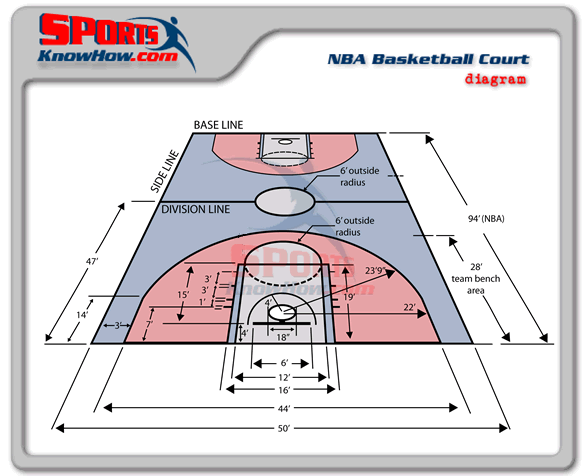
\includegraphics[width=0.80\textwidth]{NBA-court-diagram.png}
\end{figure}

We intended to place eight cameras around the court, numbered from 1 to 8 as follows.  
Camera 1 was placed at ``12 o'clock'' on the diagram, i.e. behind the clear backboard at the top of the picture
Camera 2 was placed at the top right of the diagram, in the corner.
Camera 3 was placed on the right side of the midcourt line.
The camera numbers continue increase moving clockwise around the court.

We performed this experiment at the Malkin Athletic Center (``MAC'') on Friday, November 16.  
We used a ladder and electrical tape to mount Camera 1 behind one of backboard.
The backboard on the opposite side of the court was raised up towards the ceiling,
so we were unable to obtain footage from Camera 5.
We made our best effort to orient the cameras to provide useful footage for a half-court basketball game.  
The camera orientations would need to be different to capture a full court game.
We were lucky enough that some gentlemen who were playing agreed to play
a short game on the court where we set up our cameras to assist in our experiment.
The game lasted approximately 2:26.  This might not sound like much, but it amounts to just under 4400 frames at 30 FPS.
This data set was already at a size where it put significant strain on our computational resources,
particularly those of us working on laptops.

\newpage
\section{Video Processing}
This project posed numerous practical challenges.  
Two of them were editing the video files we obtained from the cameras 
and sharing files that are far too large for GitHub with across our team.
The video cameras have SD cards, which we used to transfer our video files to a PC.
The cameras recorded in full HD (1920x1080) at 15 frames per second.
However, while the stated resolution was full HD, the image is not nearly as sharp
as a high quality camera recording at this resolution would be.
We obtained AVI files from the camera, and the first step in our workflow was to 
edit down the ~20-25 minutes of footage obtained from each camera to segments
of around 2:45 containing the game with a short buffer on either side. 
This was done using Adobe Premier video editing software.
The output of this step of the analysis was a set of 7 MPG files.
These files were very roughly time synchronized, to a resolution of around 10 seconds.
To complete the initial batch of processing, we extracted frames from these videos
using \href{https://www.ffmpeg.org/}{ffmpeg}, which is an excellent free open source tool.

\section{Finding Our Code on GitHub and Data Files on Dropbox}
All of our code for this project is available here on a public GitHub repository:
\href{https://github.com/Harvard-AM-205-Basketball/Basketball}{Harvard-AM-205-Basketball}.
While we will follow all submission instructions and upload individual Python files with this report,
the most efficient way get all of our code with the correct directory layout is to clone the repository: \\
\texttt{git clone https://github.com/Harvard-AM-205-Basketball/Basketball.git}

Our team collaborated using a combination of GitHub for source code and Dropbox for large shared files.
We created a shared folder with all of our video and audio files.  This got to be quite large.
The AVI files are about 26 GB.  The trimmed MPG files are about 8 GB.  
The fun really started when we extracted frames.  These consumed a whopping 122 GB!
(Back of the envelope: there are ~5,000 frames at 1980x1020 pixels, with 3 8 bit color channels each).
The movie has much more compression because most of the frames don't change that much.
One technique we used to manage having different folder locations was to create links in our
project directory pointing to the Dropbox folders.  
Dropbox no longer supports public folders, so the only way we know to share our data files
is to send an invitation to access the shared folder.  We are of course happy to do this.
Please be warned though that Dropbox counts the entire size of a shared folder against the
space quota of everyone who has access to it.  So if you are on a free Dropbox plan, 
sharing this folder will exhaust your space quote and leave you temporarily unable to upload files.
We are still trying to figure out if there is a better way to work collaboratively on large data files
and make them available to the public in the interests of replicable science.

The software environment for all code on this project was Python 3.6 or 3.7.
Different machines used by members of our team included a Mac laptop, a Windows Surface, 
a Windows PC, and a powerful server running Ubuntu Linux.

\section{Estimating the Background Image}
A common technique in image processing is Foreground Detection, which is equivalent to estimating the background and subtracting it out.
\footnote{\href{https://en.wikipedia.org/wiki/Foreground_detection}{Foreground Detection}}
We had two reasons to get the background image at each camera.  
First, to aid in foreground detection which we could use as input to the part of the system that would track the ball
in 2D for each camera.  Second, to aid us in calibrating the location of each camera (more on this below).
An obvious idea that can be run quickly is to take the mean of each pixel over all the frames.
This has some obvious shortcomings though, as the pixels get blurred from frames where objects are in the foreground.
We hit on the idea of estimating the median value of the R, G and B color component of each pixel.
This calculation was performed in the Python file \texttt{image\_background.py}.
There is not much going on in this file of mathematical interest.  
Getting the program to run to completion however was a nontrivial task!  
The challenge is that loading all the frames for even one camera  
consumes a prodigious amount of memory.  
While it's possible to compute the mean of all the frames by a doing a single pass through them
and accumulating the sum, we are unaware of a similar trick for the median.
In the end we got this clean but resource intensive implementation to run on an Ubuntu server that has 256 GB of ram.  
This is a good example of the kinds of challenges that cropped up somewhat unexpectedly and consumed large amounts of time.

Here are examples of the mean and median background image:
\begin{figure}[H]
\centering
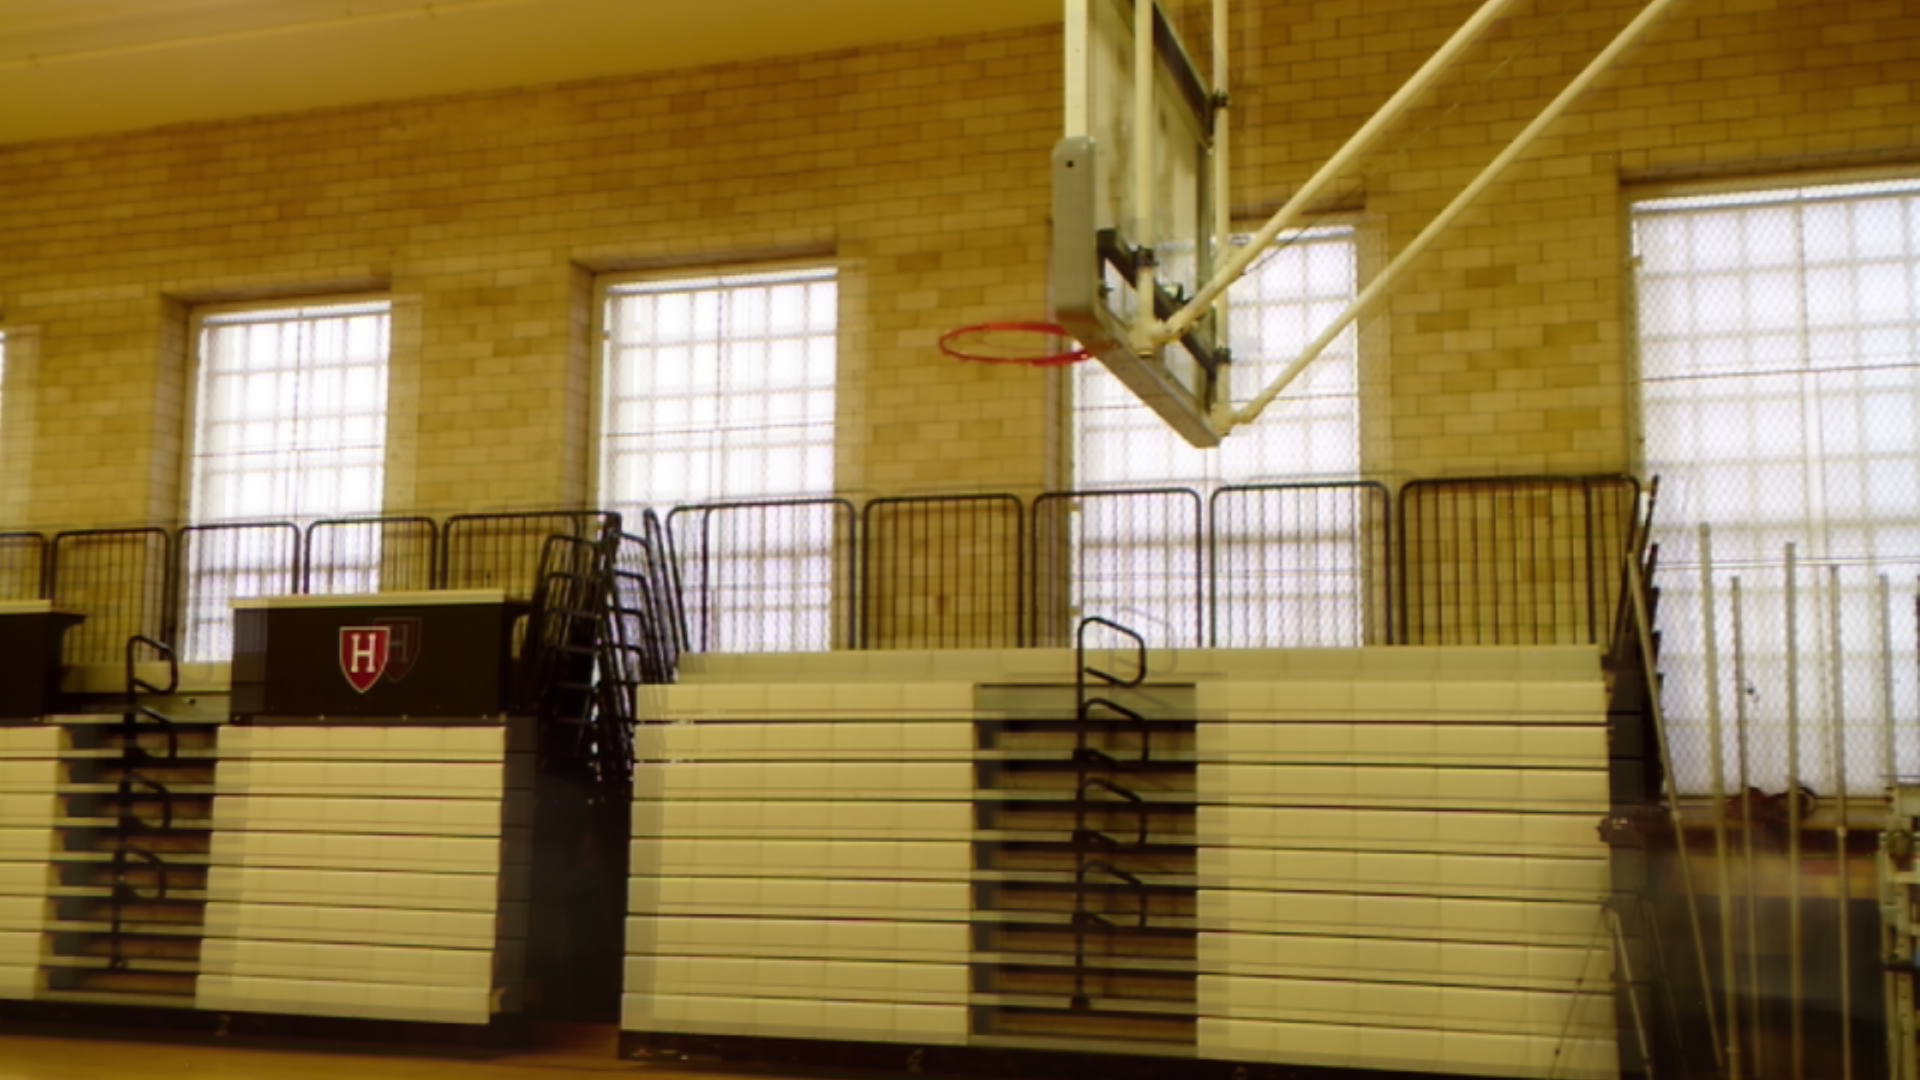
\includegraphics[width=0.80\textwidth]{Camera2_mean.png}
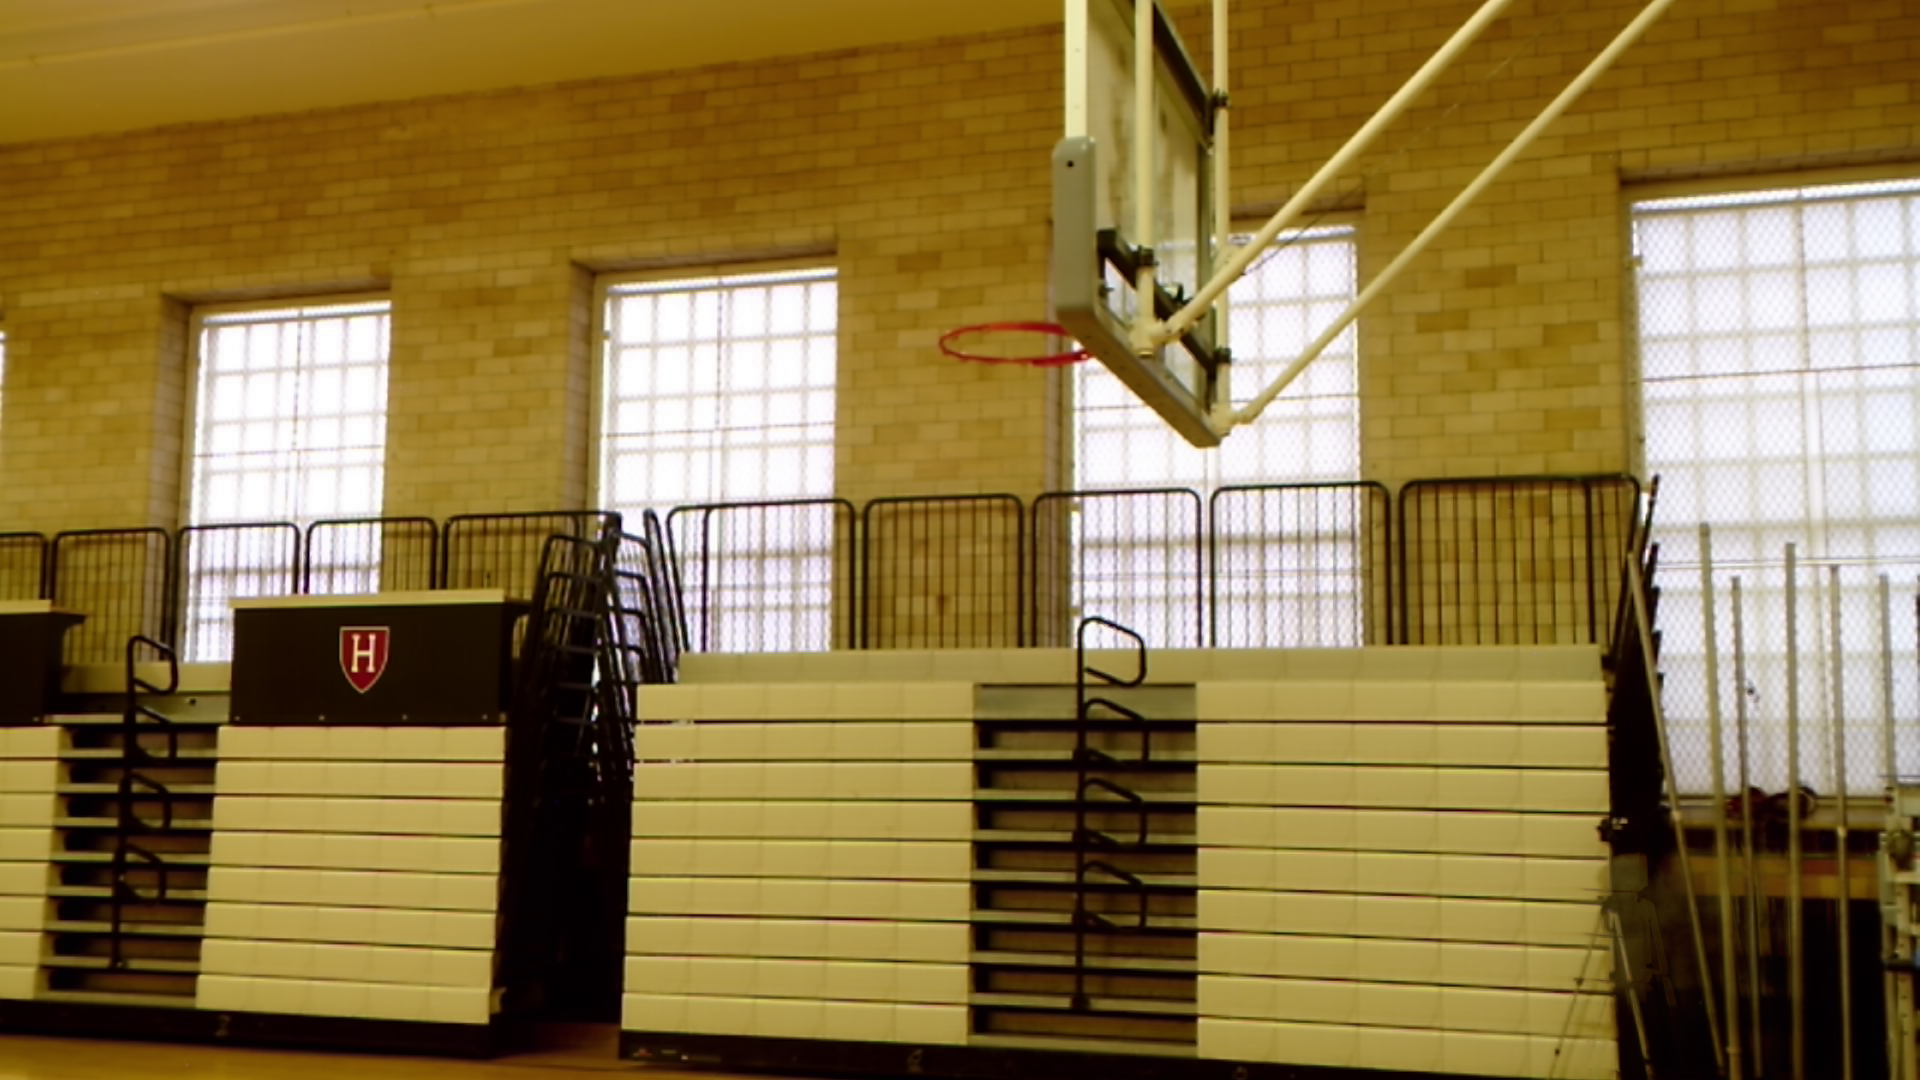
\includegraphics[width=0.80\textwidth]{Camera2_median.png}
\caption{Mean and Median Frame for Camera 2}
\end{figure}
This camera gave a good example of why we went to the trouble of estimating the median.
The mean is visibly blurry (especially around the ``H'' logo on the bleachers) and median is considerably more crisp.

\section{Synchronizing the Frames Using Audio Feeds}
In order to assemble a 3D trajectory of the ball by combining frames from different cameras,
it is necessary first to synchronize the feeds.  
This is a recurring problem in videography with multiple cameras and well studied.
Almost everyone faced with this synchronization problem tries to use the audio 
rather than the video feeds to synchronize the cameras.  There are two reasons for this choice.
First, the temporal resolution of sound is much sharper than the temporal resolution of video frames.
These cameras were only recording at 15 FPS 
(we output 30 FPS to get a bit more resolution in case two cameras were separated by ~0.03 seconds).
Sound features on the other hand have a microstructure in the thousands of Hertz.
The second reason to favor sound for synchronization is that the sound environment at the
different cameras will be much more similar than the visual environments.

We had thought that, based on the frequency with which this problem arises in different contexts,
that there would be a ``drop in'' library solution that would take two WAV files and output the lag
between them.  An extensive online search proved otherwise.  
We did identify one library called \href{https://github.com/allisonnicoledeal/VideoSync}{VideoSync}.
A half day was spent trying to get this code to run on our input files.
Unfortunately we just could not get it to run to completion.  The program would run, but would hang.
After modifying it to add progress bars and running on the monster Linux server we still had no luck.
Apparently this problem is solved in practice by highly trained video editors using expensive software,
i.e. people do it by hand.

The idea behind synchronizing two audio feeds is intuitive.
If $g(t)$ is very similar to $f(t)$ but with a lag, then $g(t) \approx f(t + \tau)$
where $\tau$ is the time lag.  So synchronizing the two feeds amounts to finding the $\tau$ that 
will maximize $\sum_t f(t) g(t - \tau)$.  This looks very similar to a 
\href{https://en.wikipedia.org/wiki/Convolution}{convolution} between $f$ and $g$.
An introductory course in Fourier Analysis cover the fact the Fourier transform of the convolution
$f * g$ is the product of the Fourier transforms of $f$ and $g$.
A practical application of this for discrete sampling problems such as this one is that convolution
can be evaluated efficiently using the Fast Fourier Transform (FFT).
One important thing to remember is that the definition of the convolution of $f*g$ is a sum over
$f(x) g(t-x)$, so we need to reverse the order of the second array before running the convolution.

An initial attempt was made to find the time lag by convolving the two audio signals 
(i.e. sound waves loaded from WAV files).  
We created a simple test case by taking the audio from one camera and applying lags of 1.0 and 3.0 seconds to it.
The convolution based approach (evaluate the convolution, then run \texttt{np.argmax} to find the lag with maximum overlap)
worked flawlessly on this test data.  But when it was tried on the actual audio feeds, it failed completely.  
It was way off, and the correlations between the signals was very low, in the vicinity of 0.02.
The problem is that the sound waves oscillate very rapidly, and small differences in the sound environments
at the cameras cause the signals to sometimes line up and other times not to line up.
The test case worked well because the dummy test data kept both the micro and macro structure of the waves.
But while the macro structure of the sound at each camera (as perceived by a person) was very similar,
the waves didn't line up that tightly.

The second attempt had two phases and was successful.  The first phase was very low tech:
by listening to the seven WAV files, we estimated the lags between them to a resolution of approximately one second.
This was done by noting the times when audible phrases were spoken.  
(``I'm going to check the cameras'' and ``oh, dude!'').
The signals were approximately aligned using these preliminary lags.
We then applied a Fast Fourier Transform to the signals to estimate the sound environment during that window.
The audio feed was sampled at 48,000 Hz.  
We referred to the discussion and code in 
\href{https://engineersportal.com/blog/2018/9/13/audio-processing-in-python-part-i-sampling-and-the-fast-fourier-transform}{audio processing in python}
when implementing this solution.
We selected a window size of $2^{12} = 4096$ pulses, corresponding to 0.0853 seconds.
(The FFT is most efficient when the window size is a power of 2; a sound window of roughly 0.1 seconds is a useful guideline.)
These windows were sampled with a spacing of 1024 pulses, corresponding to a temporal resolution of 0.0213 seconds. 
This is small enough compared to the 0.033 seconds between frames at 30 FPS that if done correctly,
it should allow us to synchronize to the nearest frame.  
An audio feed of 165 seconds was thus processed into approximately 7,800 overlapping windows.
Each window was characterized by a vector of 4096 numbers from the FFT output.
Here is a visualization of the sound frequency profile at camera 1 on the 100th bucket (about 2.0 seconds):
\begin{figure}[H]
\center
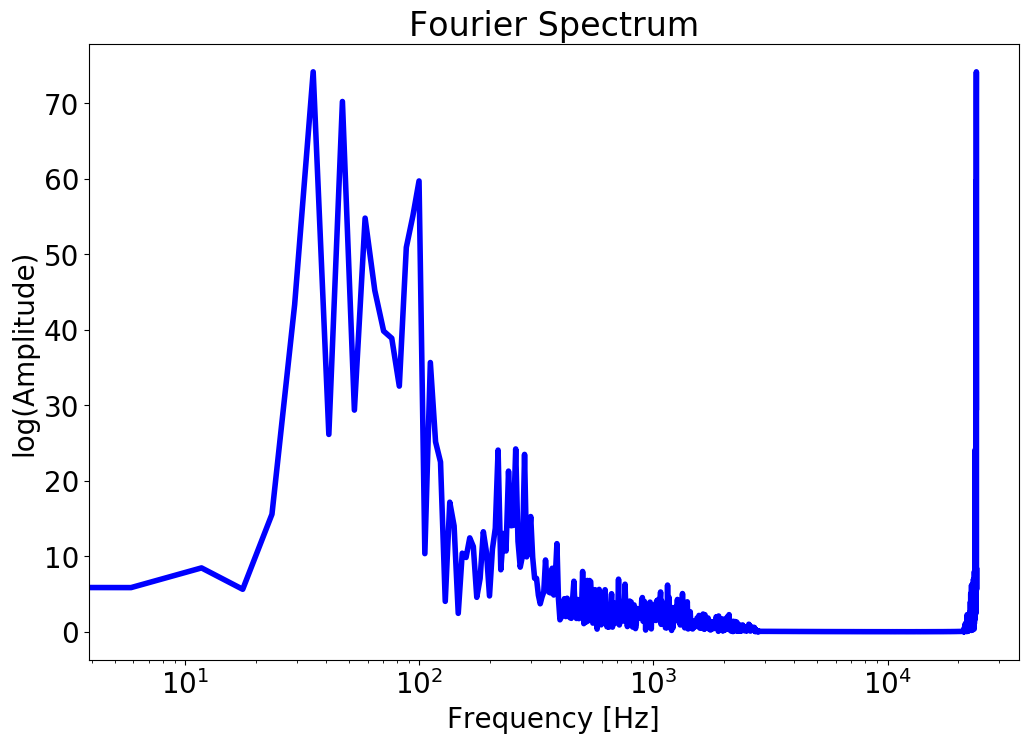
\includegraphics[width=0.80\textwidth]{fourier_spectrum.png}
\end{figure}

After each sound signal is converted to a Fourier spectrum, 
the spectra are then convolved against each other to find the lag between signals.
In this case, rather than taking the dot product of two scalar functions of time, 
we are taking the dot product of two vectors containing the amplitude of the 
signal at different frequencies on the spectrum.  
This approach was successful.  It resolved the time delays to a resolution of 0.02 seconds,
sufficient to synchronize the frames to the nearest frame number.
We generated a 7x7 skew symmetric matrix of estimated time lags.
The rows were averaged to form a composite estimate of the lags between cameras.
As a quality metric, we generated a 7x7 correlation matrix of the spectra after
they were synchronized.  We then extracted the largest eigenvalue.
For perfectly synchronized signals, the correlation matrix would be all 1s,
and the first eigenvalue would be 7.  This run achieved a first eigenvalue of 4.742.

All code used to synchronize the audio feeds can be found in the file \texttt{audio\_synchronize.py}.
The function \texttt{wav\_to\_freq} converts a WAV audio file to a Fourier spectrum using the FFT.
The function \texttt{synchronize\_spectra} finds the time lag between two spectra by convolving one
against the reversal of the other and taking the argmax of the result.
The function \texttt{make\_synch\_matrix} builds an 7x7 matrix of estimated lags.
Even though there are only 6 degrees of freedom in this problem , 
we estimate all 42 entries and then average the rows to maximize the accuracy of the measurement.
The outputs of the synchronization calculation are in the test file \texttt{synchronization\_output.txt}
in the \texttt{calculations} directory of our repository.

Of course the proof of the pudding is in the eating.  
Here are images from six of the seven cameras of the first ostensibly synchronized frames:
\begin{figure}[H]
\center
\includegraphics[width=1.00\textwidth]{synced_frames.png}
\end{figure}

If you pay close attention to the ball, you can see that in all six frames, the gentleman
in the gray longsleeve shirt with a goatee is dribbling the ball with a high stroke, 
and the ball is close to its apex.  This is particularly clear on the first three views
if you start at the top left and read them like a page in a book (right, then down).
We claim this is evidence that the audio synchronization was accurate to the nearest frame!

\newpage
\section{Transforming 3D World Coordinates to Pixel Locations}

\subsection{Conventions}
Coordinates in the world frame will be denoted as $(U, V, W)$. Coordinates in the camera frame will be denoted as $(X, Y, Z)$. 
Coordinates in the 2D image plane will be denoted as $(x, y)$. Pixel coordinates will be denoted as $(u, v)$. \\

The court has the following dimensions and coordinate system 
(all units are in FEET for this project because US basketball court sizes are standardized in feet, not meters). 
Note that we are centering the world coordinate system at the center of the court and that the $w$ axis points towards the ceiling.

\begin{figure}[H]
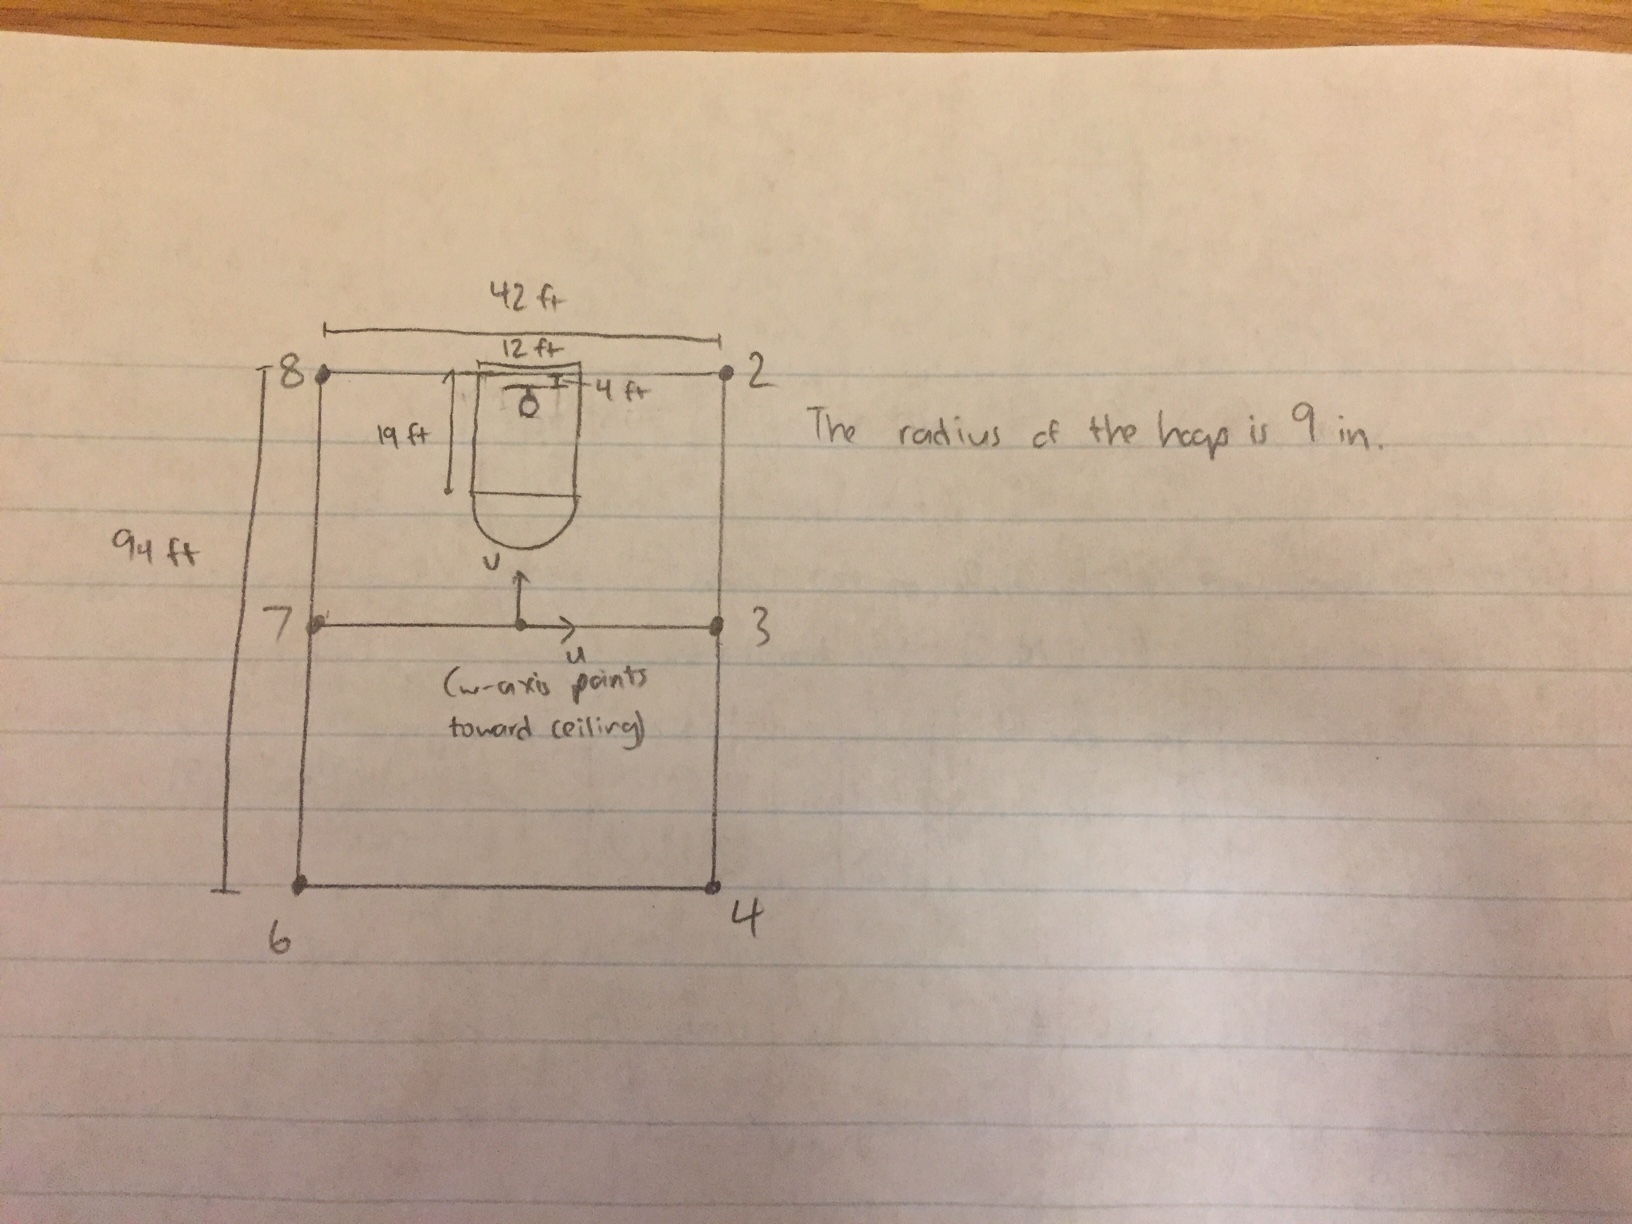
\includegraphics[scale=0.25]{Court_Diagram}
\centering
\caption{A diagram of the MAC basketball court with dimensions}
\end{figure}

For the camera frame, we will adopt the convention that the $Z$ axis points in the direction that the camera is pointing. 
See the following diagram, where the rectangular prism represents the camera:

\begin{figure}[H]
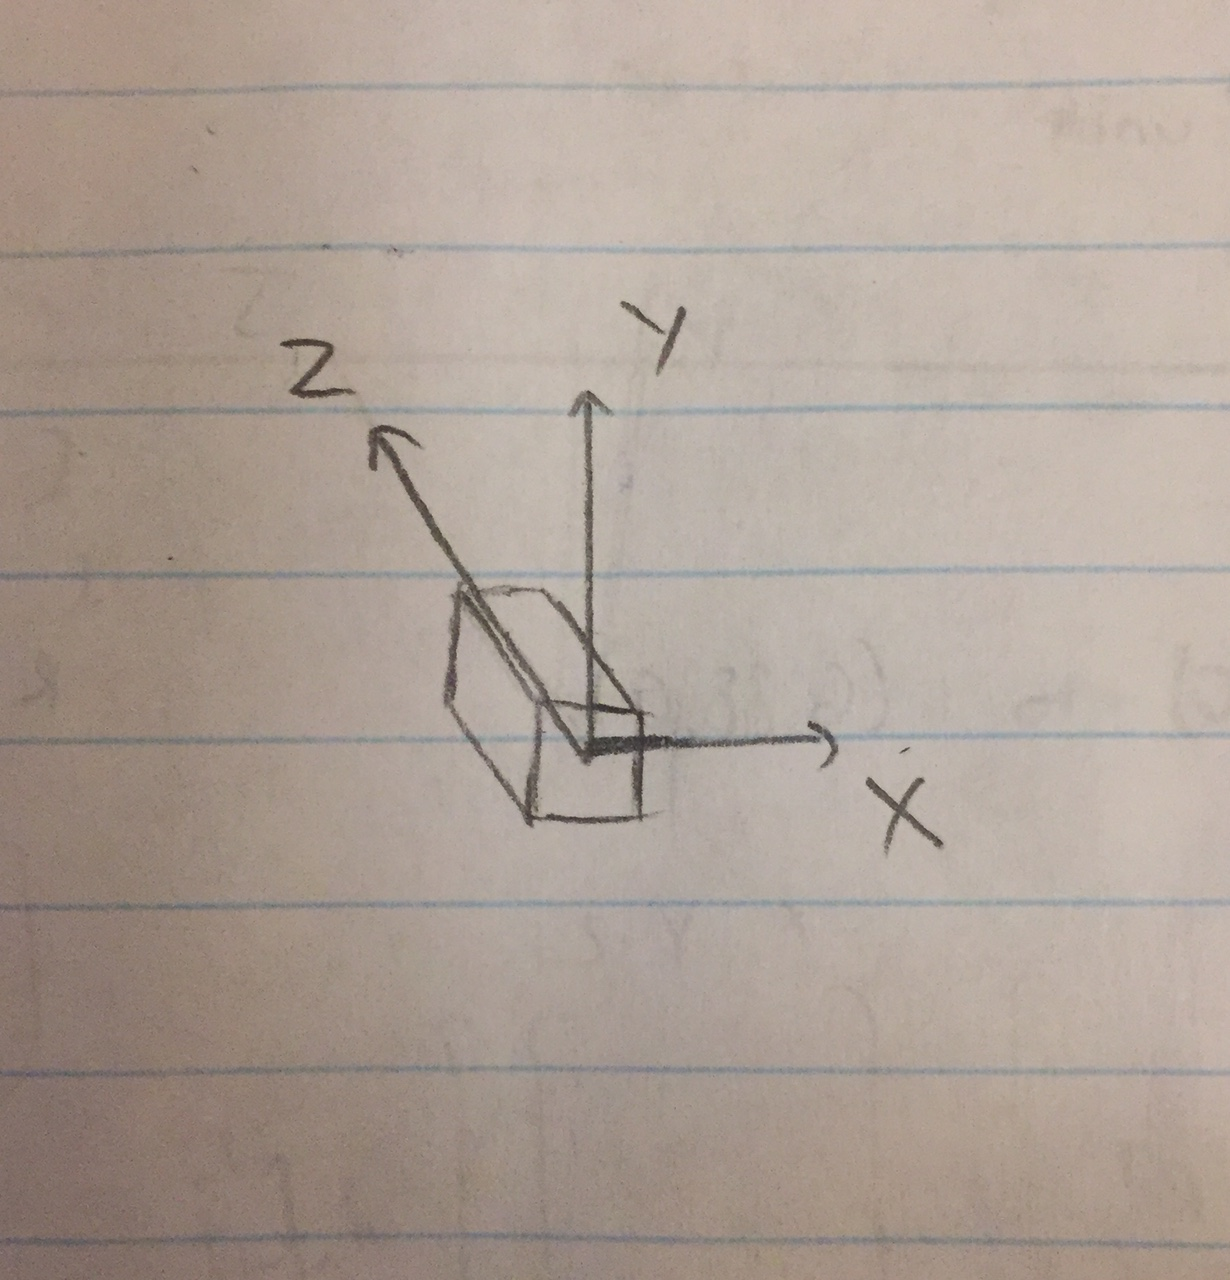
\includegraphics[scale=0.1]{Camera_Coordinates}
\centering
\caption{A hand sketched representation of the camera coordinate system}
\end{figure}

The image coordinate system has the origin at the center of the image, with the $x$-axis pointing to the right and the $y$-axis pointing up (i.e. standard conventions). 
The pixel coordinate system has $(0, 0)$ representing the pixel in the top left corner. 
Also note that it is represented as an array in Python with the first coordinate representing the row of the pixel 
(so the $u$ axis points down and corresponds to the image $-y$ axis) and the second coordinate representing the column 
(so the $v$ axis points to the right and corresponds to the image $x$ axis).

\subsection{World to Camera}
To get from world coordinates to camera coordinates, we must perform a translation and then a rotation. 
Let the camera be placed at location $\bm{C}$ (denoting a vector) in the world frame, and let the rotation matrix be $R$. 
Since the rotation matrix $R$ is designed to go from the world to the camera coordinate system, $R^{T}$ is designed to go from the camera to the world. 
Thus, the first column of $R^{T}$ should represent the camera $X$-axis in world coordinates, the second column should represent the $Y$-axis, 
and the third column should represent the $Z$-axis. 
In terms of $R$, we see that the first \textit{row} of $R$ must be equivalent to the camera $X$-axis in world coordinates, etc. \\

In practical terms, it is relatively easy to estimate what the camera $Z$-axis is in world coordinates. 
By looking at one frame and identifying the center pixel (I used MS Paint for this), we can identify where in the world coordinate system the camera is pointing. 
The easiest way to do this is to consider where the ray pointing down the camera $Z$-axis hits a solid object. 
For example, if the center pixel is on the rim or the backboard, we can write a vector representing where that point is in relation to the camera position. 
We then normalize the vector to get the third row of $R$. \\

To get the $X$-axis, we rely on the assumption that the camera $X$-axis has a $W$-coordinate of 0 in the world frame (i.e. that it is parallel to the ground). 
This is a reasonable assumption because we start with the camera pointed parallel to the ground. 
When we tilt the camera slightly upwards, we don't rotate it in any other way, so the $X$-axis stays stationary while the $Z$ and $Y$ axes rotate (see Figure below). 
Thus, we look at the first two world coordinates of the camera $Z$-axis, flip the order of the coordinates, 
and change one sign (we flip the sign of the $U$-coordinate so that the $X$ axis points to the right). 
This ensures that the $X$ and $Z$ axes are orthogonal (have a dot product of 0). \\

\begin{figure}[H]
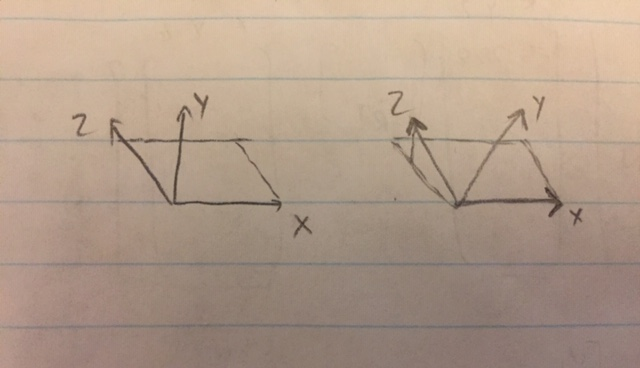
\includegraphics[scale=0.6]{Rotation_Diagram}
\centering
\caption{Why the camera $X$ axis is parallel to the ground}
\end{figure}

Finally, to get the $Y$-axis, we first normalize the $X$ and $Z$ axes, and then take the cross product of $X$ and $Z$. 
We make sure $X$ comes first so that the $Y$-axis points in the right direction by the right hand rule. 
We put our three unit vectors together and we have a rotation matrix $R$! 
We can now relate camera coordinates to world coordinates:

\[ \bm{P}_{C}=R(\bm{P}_{W}-\bm{C}) \]

\subsection{Camera to Image}
The key idea is that the ``image plane'' is an imaginary plane $f$ units down the $Z$-axis of the camera, where $f$ is the focal length. 
To get the image plane coordinates, we use similar triangles and scale down a point that is $Z$ units away to a plane that is $f$ units away. We get:
\begin{align*}
x&=\frac{f}{Z}X \\
y&=\frac{f}{Z}Y \\
\end{align*}

Note: Some sources like to use ``homogeneous coordinates'' so that we can write a matrix equation
 $\begin{bmatrix} x' \\ y' \\ z' \end{bmatrix}=\begin{bmatrix} f & 0 & 0 & 0 \\ 0 & f & 0 & 0 \\ 0 & 0 & 1 & 0 \end{bmatrix}\begin{bmatrix} X \\ Y \\ Z \\ 1 \end{bmatrix}$. 
 
 Then $(x', y', z')=(Xf, Yf, Z)$ and $(x, y)=(\frac{x'}{z'}, \frac{y'}{z'})$. 

\begin{figure}[H]
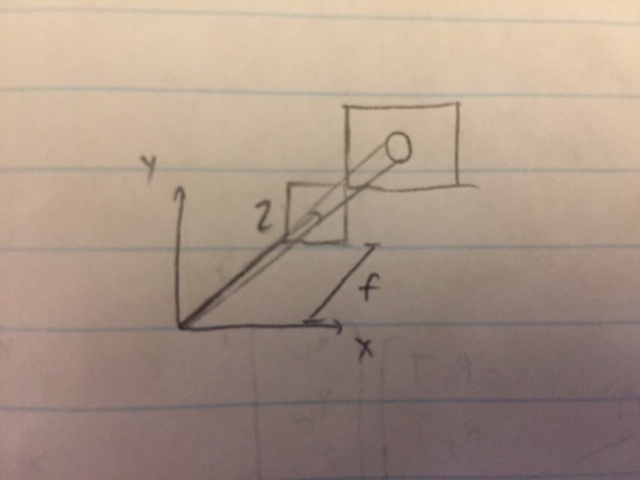
\includegraphics[scale=0.6]{Image_Plane}
\centering
\caption{Projection onto image plane}
\end{figure}

\subsection{Image to Pixel}
To transform from image to pixel, we have to divide the image $x$ coordinate by the width of a pixel and the image $y$ coordinate by the height of a pixel. This will tell us how many pixels away a point in the image is from the center of the image. Let the width of a pixel by $s_{x}$ and the height of a pixel by $s_{y}$. Also, note that we must negate the image $y$ coordinate because the pixel $u$ axis points down instead of up. Right now we have $u=-\frac{y}{s_y}, v=\frac{x}{s_x}$. However, we have to add $\frac{1080}{2}=540$ to $u$ and $\frac{1920}{2}=960$ to $v$ so that the pixel $(0,0)$ is in the top left corner. The exact numbers come from the fact that each frame is 1080 by 1920 pixels.

\begin{align*}
u&=-\frac{y}{s_{y}}+540 \\
v&=\frac{x}{s_{x}}+960
\end{align*}

\begin{figure}[H]
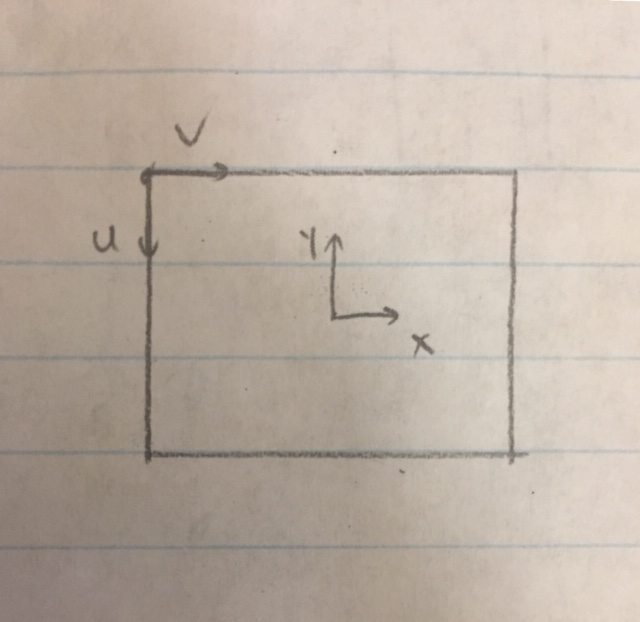
\includegraphics[scale=0.3]{Pixel_Coordinates}
\centering
\caption{Pixel coordinates vs. image coordinates}
\end{figure}

\subsection{Extrinsic vs. Intrinsic Parameters}
The rotation matrix $R$ and the position of the camera $\bm{C}$ are considered \textbf{extrinsic parameters} in the sense that we set them. We can also obtain good estimates of what they are without doing any algebra or optimization. On the other hand, the focal length $f$ and the pixel size $s_{x}$ by $s_{y}$ are \textbf{intrinsic parameters}, which means that they are properties of the camera. While the focal length is easily obtainable from the SOSUN website (7.36 mm unzoomed), the pixel size is unknown. However, we can estimate it using least squares! \\

We know the world coordinates of several points on the court, such as the free-throw rectangle and the white square on the backboard. Given our estimates for all of the other parameters, we can solve for the image coordinates $(x, y)$ of these points relatively easily. We can also identify the pixel coordinates $(u, v)$ of these points relatively accurately by examining a given frame (the camera is stationary). We have the equations:

\begin{align*}
v&=\frac{x}{s_{x}}+960 \\
u&=-\frac{y}{s_{y}}+540
\end{align*}

And we can write this as a matrix equation $\begin{pmatrix} v-960 \\ u-540 \end{pmatrix}=\begin{pmatrix} x & 0 \\ 0 & -y \end{pmatrix}\begin{pmatrix} \frac{1}{s_x} \\ \frac{1}{s_y} \end{pmatrix}$. We have many points where we know $(x, y)$ and $(v, u)$, so we can make this a least-squares problem where we solve for $\frac{1}{s_x}, \frac{1}{s_y}$!

\[\begin{pmatrix} v_1-960 \\ u_1-540 \\ v_2-960 \\ u_2-540 \\ \hdots \end{pmatrix}=\begin{pmatrix} x_1 & 0 \\ 0 & -y_1 \\ x_2 & 0 \\ 0 & -y_2 \\ \hdots & \hdots \end{pmatrix}\begin{pmatrix} \frac{1}{s_x} \\ \frac{1}{s_y} \end{pmatrix}\]

Assuming we have estimated all of the other parameters correctly, we should be able to get accurate numbers for $s_x, s_y$, allowing us to transform any point on the court into pixels.

\subsection{An example, using Camera 3}
Using Camera 1, we can see that Camera 3 is outside of the court, slightly behind and to the right of where it is supposed to be on the diagram. 
We also know that it is on a 5-foot high tripod. 
Using the diagram of the court, we estimate that its position relative to the world-frame origin is $\bm{C}=(22, -1.5, 5.2)$. \\

Next, we compute the rotation matrix. The center pixel of frame 20 (we could choose any frame) lies directly below the front of the rim. 
If we draw a line from the rim to the ground (using MS Paint), we estimate that the camera is pointed about 2 feet below the front of the rim. 
The point 2 feet below the front of the rim has world coordinates $(0, 41, 8)$, so the camera $z$-axis points in the direction $(-22, 42.5, 2.8)$.
 Our assumption is that the $x$-axis has a 3rd coordinate of 0 and points towards the northeast, so it must be of the form $(42.5, 22, 0)$ 
 in order to be orthogonal to $z$ (of course, it could be any scalar multiple of this). 
 In Python, we normalize our two vectors and then take $x\times z$ to get the $y$-axis. 
 Our rotation matrix is $R=\begin{pmatrix} \vec{x}_n \\ \vec{y}_n \\ \vec{z}_n \end{pmatrix}$ where the $n$ subscript indicates that our vectors are normalized to have norm 1. \\

Note that our choice to look at the point 2 feet below the front of the rim was arbitrary, as the camera $z$-axis represents a ray. 
However, it was the easiest choice because it was a point on the ray with coordinates that were relatively easy to estimate. \\

From here, all we need to do is solve the least-squares point for the pixel size $(s_x, s_y)$. 
For our ``known'' points, we take the free throw rectangle and the white box on the backboard. 
The four corners of the free throw rectangle are $(-6, 28, 0), (-6, 47, 0), (6, 47, 0), (6, 28, 0)$ in world coordinates, 
and the four corners of the box on the backboard are $(-1, 43, 10), (-1, 43, 11.5), (1, 43, 11.5), (1, 43, 10)$. 
We also consider some intermediate points on the free throw rectangle (I used all of the points with integer coordinates). 
Using Python, we can create a $N$ by 3 matrix with the world coordinates of these points. 
With the parameters we already know, we can construct the 2D image plane coordinates of these points. \\

We can also get the pixel coordinates of all of our points with reasonable accuracy by looking at the photo in MS Paint or similar software. 
I did this by getting the pixel coordinates of the corners and using linspace. 
Now that we have our pixel coordinates and our 2D image plane coordinates for all of our points, we solve the least squares problem for $s_x$ and $s_y$. 
Our final step in Python is to use our estimated values of $s_x$ and $s_y$ to complete the transformation and color the pixels corresponding to our real-world points 
(in this case, the free throw rectangle and the white box).

\subsection{Python Implementation of Coordinate Transforms}
The file \texttt{camera\_transform} implements all of these formulas in a modular form.
Function \texttt{cam2pix} converts coordinates $(x, y)$ in the local image plane to integer pixel values $(u, v)$.
Function \texttt{make\_transforms} takes as inputs 
\texttt{cam\_pos}, the position of the camera in the world frame, and
\texttt{cam\_point}, the position of \textit{any} object that the center of the camera is pointing at.
This function is a ``factory'' that makes a pair of transformers returning $(x, y)$ and $(u, v)$ coordinates.

\bigskip
\subsection{Resources}
\url{http://www.cse.psu.edu/~rtc12/CSE486/lecture12.pdf} \\
\url{http://www.cse.psu.edu/~rtc12/CSE486/lecture13.pdf} \\
\url{https://courses.cs.washington.edu/courses/cse455/09wi/Lects/lect5.pdf} \\
\url{https://www.cs.utah.edu/~srikumar/cv_spring2017_files/Lecture2.pdf} \\
\url{http://www.cs.toronto.edu/~jepson/csc420/notes/imageProjection.pdf} \\
\url{http://people.scs.carleton.ca/~c_shu/Courses/comp4900d/notes/camera_calibration.pdf} \\
\url{http://www.cs.ucf.edu/~mtappen/cap5415/lecs/lec19.pdf} \\
\url{https://www.cse.unr.edu/~bebis/CS791E/Notes/CameraParameters.pdf} \\

\newpage
\section{Visual Calibration of Camera Position and Orientation}
It is possible to confirm a camera calibration visually.  
The idea is straightforward, though as usual on this challenge, the devil is in the details.
We know where various prominent visual features on a basketball court are located in the
``world frame'' coordinate system of the court.  
For instance, we know the court should be 94 feet long and that the rim should be exactly 10 feet over the ground.
The idea is to produce arrays of 3D points on these objects, and then transform them to pixel locations.
We can than ``annotate'' an image by overlaying the predicted pixel positions of visual landmarks on the image.
If the calibration is correct, we will paint virtual lines on the perimeter, key, backboard, etc.

The Python file \texttt{basketball\_court.py} computes coordinates for a series of visual landmarks on a
basketball court including the perimeter, midcourt line, restraining circle at the center of the court,
the ``key'', and the three point arc.  Here is a plot of the XY plane:
\begin{figure}[H]
\center
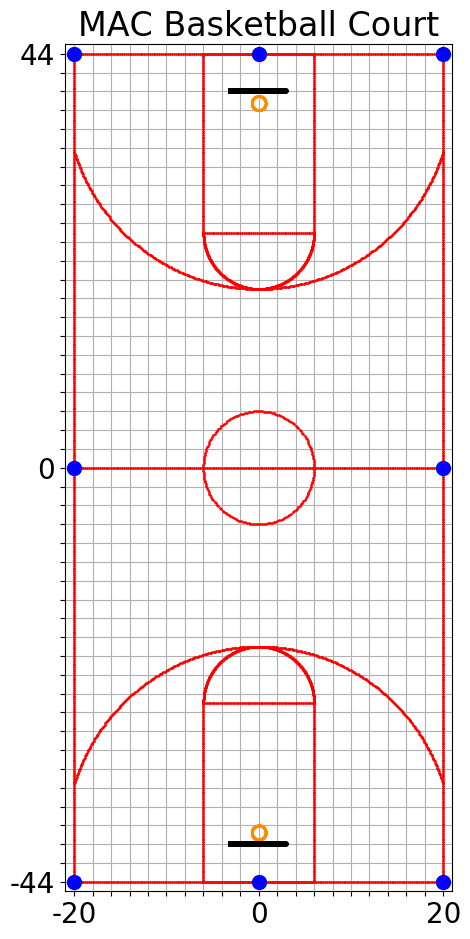
\includegraphics[width=0.68\textwidth]{court_lines.png}
\end{figure}

A careful observer will note that this figure does not quite match up with an NCAA regulation basketball court.
This is not an error in the Python code!  It turns out that the court we used for our experiment at the MAC...
is not a regulation basketball court.  Not even close.  It's far narrower than a regulation court.
That's why the widest edge of the three point arc is practically flush against the perimeter line.
With the benefit of hindsight, it would have been much easier for us if we'd located a court with standard dimensions.
However we needed to do quite a bit of setup work, and it might not have been feasible to locate another court
where the staff and players would be so accommodating of a science experiment encroaching on the athletic realm.

At the top of the file, global variables are set with various dimensions of the court.
The functions \texttt{make\_line}, \texttt{make\_polygon}, 
% \texttt{make\_arc}, and \texttt{make_circle}
assemble arrays of 3D vectors of sample points on objects of these types.
The function \texttt{make\_court\_lines} is the workhorse, generating both the lines plotted above
which appear on the floor of the court, but also features corresponding to a vertical line from the
floor to the base of the rim; the small and large white rectangle painted on the backboard;
and the rim.

Here is a visual demonstration to accompany the earlier discussion of the calibration of Camera 3:
\begin{figure}[H]
\center
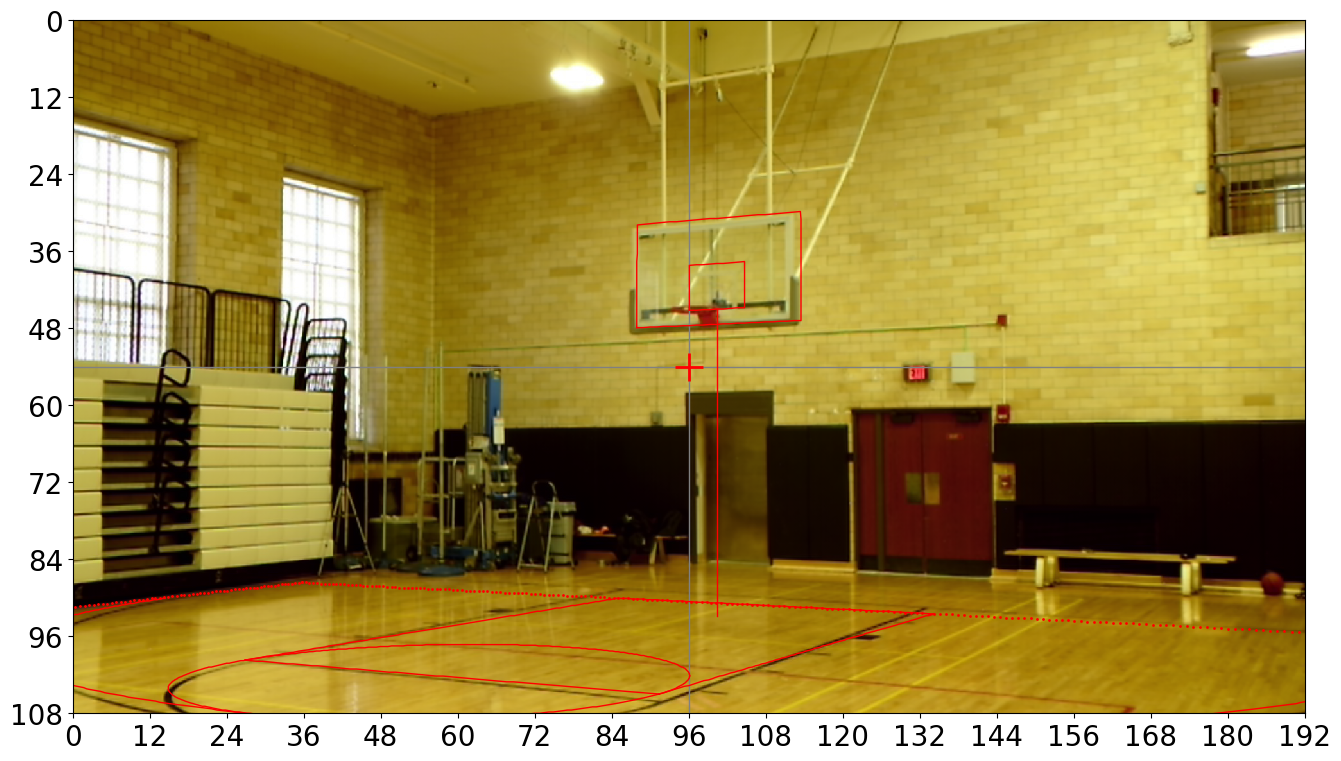
\includegraphics[width=1.00\textwidth]{Camera3_calibration.png}
\end{figure}

The red pixels painted in correspond to the projected locations of the key,
three point arc, backboard, and a vertical line to the bottom of the hoop.
The red plus sign represents the center of the camera and is intended as an aid
to estimating a point $z$ that the camera points towards.
This picture gives us a sense of both what has been accomplished and what is left to do.
The overlap between the projected pixels and corresponding landmarks on the photo is quite tight
and a convincing demonstration that all of these calculations are basically correct.
But, they're also not exactly right.  We spent a lot of time manually fiddling the calibration parameters
and weren't able to improve materially on this estimate.
When we started the project, we had hoped we could automate this process, but doing the visual
processing to extract the pixels corresponding to the landmarks has been too labor intensive for us
to automate this calculation in the available time.  
Automating the calibration is one of our top areas where we would like to improve in the future
if we continued working on this problem.


\end{document}